\section*{6.2 Parallelization of Minimax}
\subsection*{What is a good decomposition strategy of the workload to get load balance?}
We decided to distribute the tasks of evaluating the topmost layer of nodes in a roundrobin fashion between the processes. For more sophisticated algorithms like alpha-beta-pruning, this is obviously not a very good design, but for minimax, this leads to a reasonable load balance, because everyone of those nodes is exactly the same amount of work.

\subsection*{What is the speedup you get for the different scenarios from subtask 1, related to the performance metric "evaluations/sec", using 2,4,6,8 processes?}


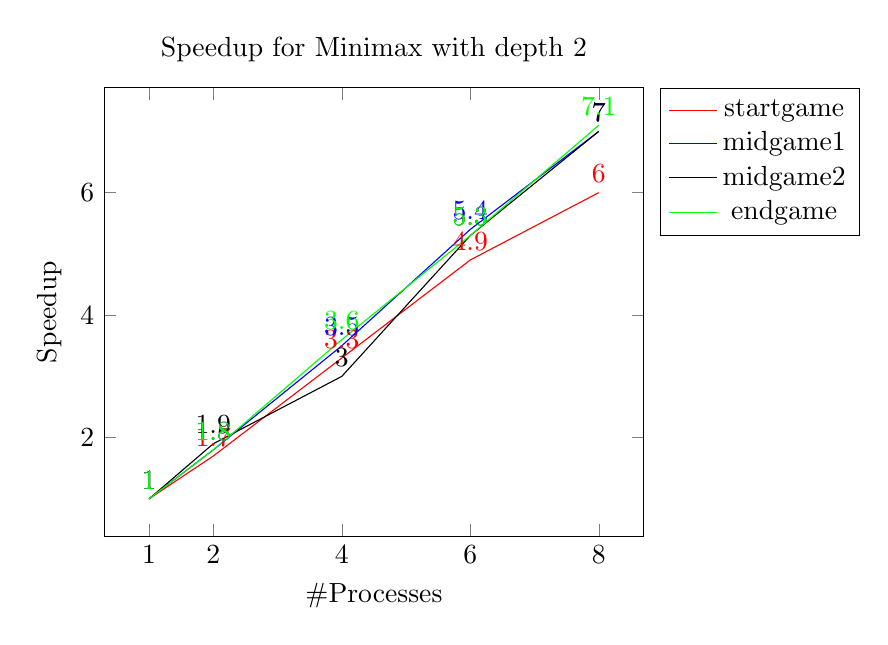
\begin{tikzpicture}
  \begin{axis}[
      legend style={cells={align=left}},
      xtick={1, 2, 4, 6, 8},
      xlabel=\#Processes,
      ylabel=Speedup,
      title=Speedup for Minimax with depth 2,
      legend pos = outer north east,
      nodes near coords,
      scaled ticks = false,
      y tick label style={
        /pgf/number format/.cd,
	fixed,
        fixed zerofill,
	precision=0,
        /tikz/.cd
      },
      no markers]
    \addplot[color=red] coordinates {
      (1,1)
      (2,1.7)
      (4,3.3)
      (6,4.9)
      (8,6)
    };
    \addplot[color=blue] coordinates {
      (1,1)
      (2,1.8)
      (4,3.5)
      (6,5.4)
      (8,7)
    };
    \addplot[color=black] coordinates {
      (1,1)
      (2,1.9)
      (4,3)
      (6,5.3)
      (8,7)
    };
    \addplot[color=green] coordinates {
      (1,1)
      (2,1.8)
      (4,3.6)
      (6,5.3)
      (8,7.1)
    };
    \legend{startgame, midgame1, midgame2, endgame}
  \end{axis}

\end{tikzpicture}
  \\
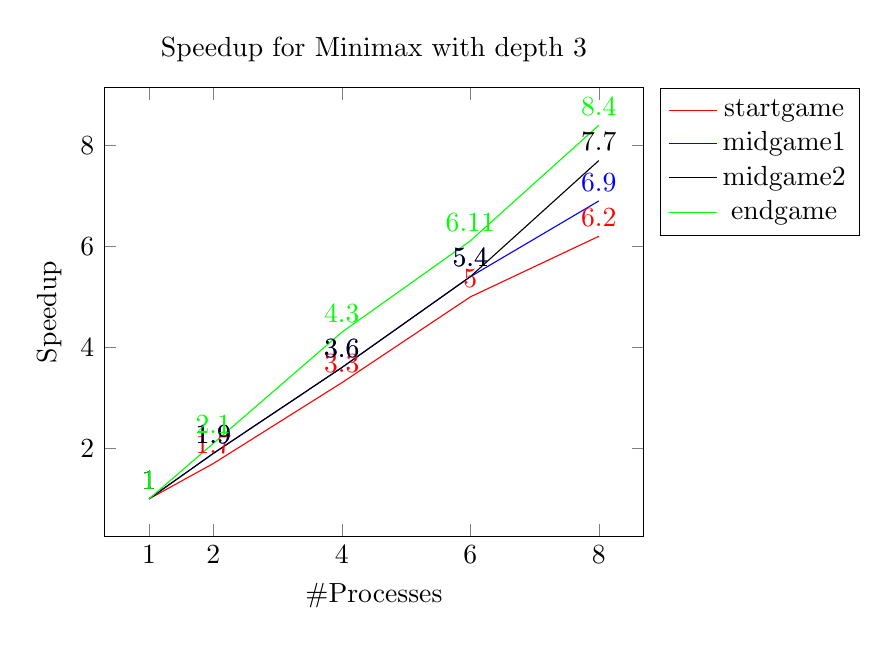
\begin{tikzpicture}
  \begin{axis}[
      legend style={cells={align=left}},
      xtick={1, 2, 4, 6, 8},
      xlabel=\#Processes,
      ylabel=Speedup,
      title=Speedup for Minimax with depth 3,
      legend pos = outer north east,
      nodes near coords,
      scaled ticks = false,
      y tick label style={
        /pgf/number format/.cd,
	fixed,
        fixed zerofill,
	precision=0,
        /tikz/.cd
      },
      no markers]
    \addplot[color=red] coordinates {
      (1,1)
      (2,1.7)
      (4,3.3)
      (6,5)
      (8,6.2)
    };
    \addplot[color=blue] coordinates {
      (1,1)
      (2,1.9)
      (4,3.6)
      (6,5.4)
      (8,6.9)
    };
    \addplot[color=black] coordinates {
      (1,1)
      (2,1.9)
      (4,3.6)
      (6,5.4)
      (8,7.7)
    };
    \addplot[color=green] coordinates {
      (1,1)
      (2,2.1)
      (4,4.3)
      (6,6.11)
      (8,8.4)
    };
    \legend{startgame, midgame1, midgame2, endgame}
		\end{axis}
\end{tikzpicture}

We noticed a superscalar speedup for position endgame while searching with depth3 which was reproducable. However, we do not know the reason for that.



\subsection*{When and why does the achievable speedup depend on the current game position?}
The game position has a huge effect on the shape of the game tree. Early on, nearly every leave has the same depth (i. e. \_maxdepth), while in later situations, there might be some leaves with shorter depths, because an earlier move would end the game. As those effects depend largely on the setting of \_maxdepth, which we were not able to run too high because of the bad performance of our algorithm, above numbers do not necessarily show that. But this issue should still exist with alpha-beta-pruning, so we should come up with a more reasonable decomposition.
